\begin{figure}[H]
    \centering
    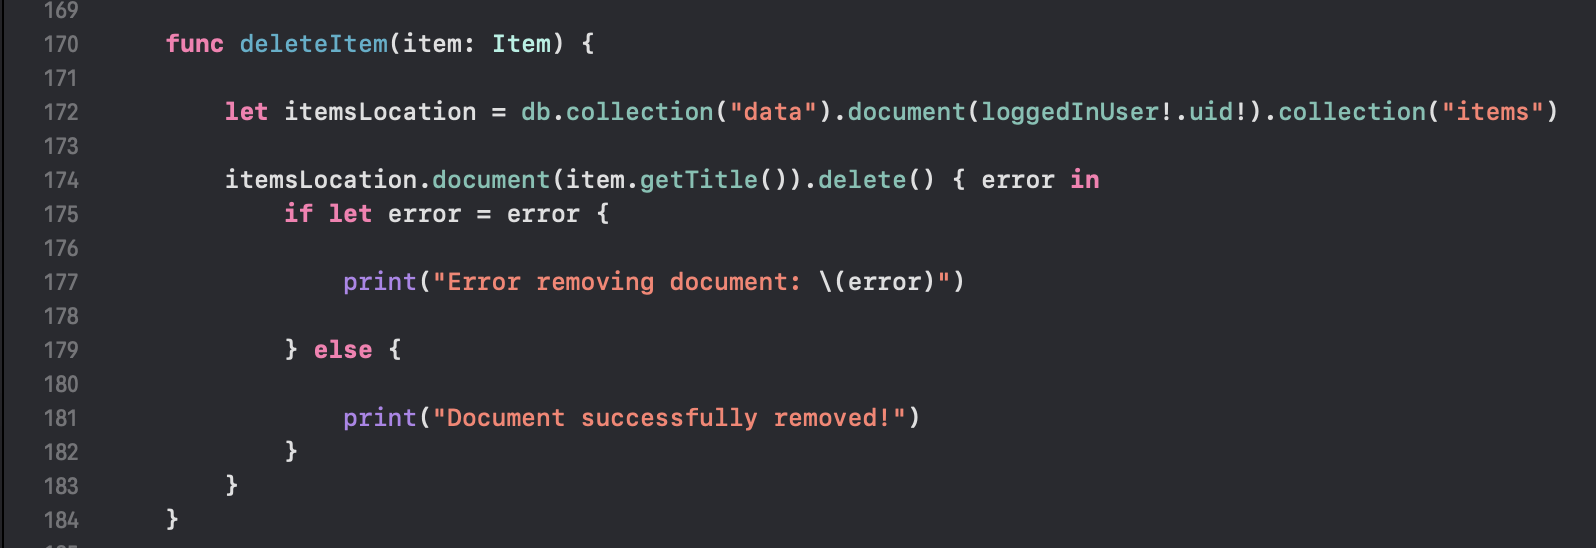
\includegraphics[width=\textwidth]{./graphics/Implementation/Dashboard/firebasesession1.png}
    \caption{deleteItem() function defined in FirebaseSession class.}
    \label{fig:firebasesession1_dashboard}
\end{figure}

\begin{figure}[H]
    \centering
    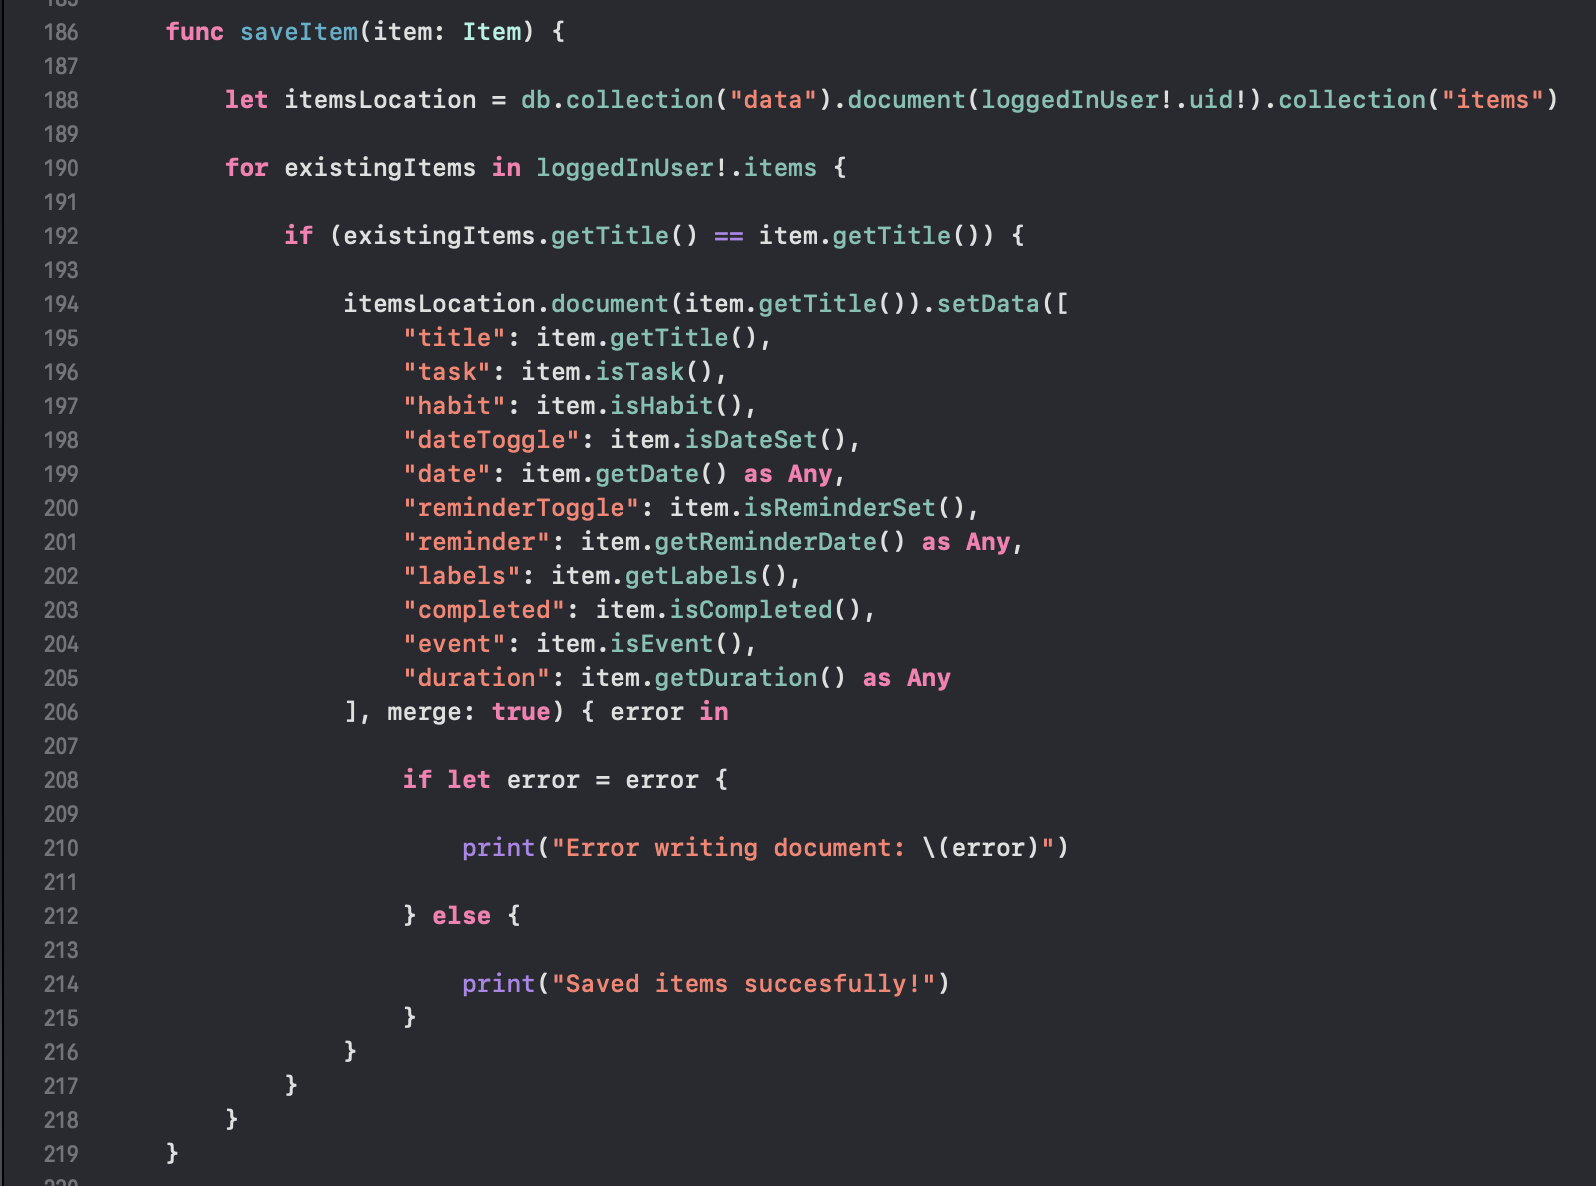
\includegraphics[width=\textwidth]{./graphics/Implementation/Dashboard/firebasesession2.png}
    \caption{saveItem() function defined in FirebaseSession class.}
    \label{fig:firebasesession2_dashboard}
\end{figure}

\begin{figure}[H]
    \centering
    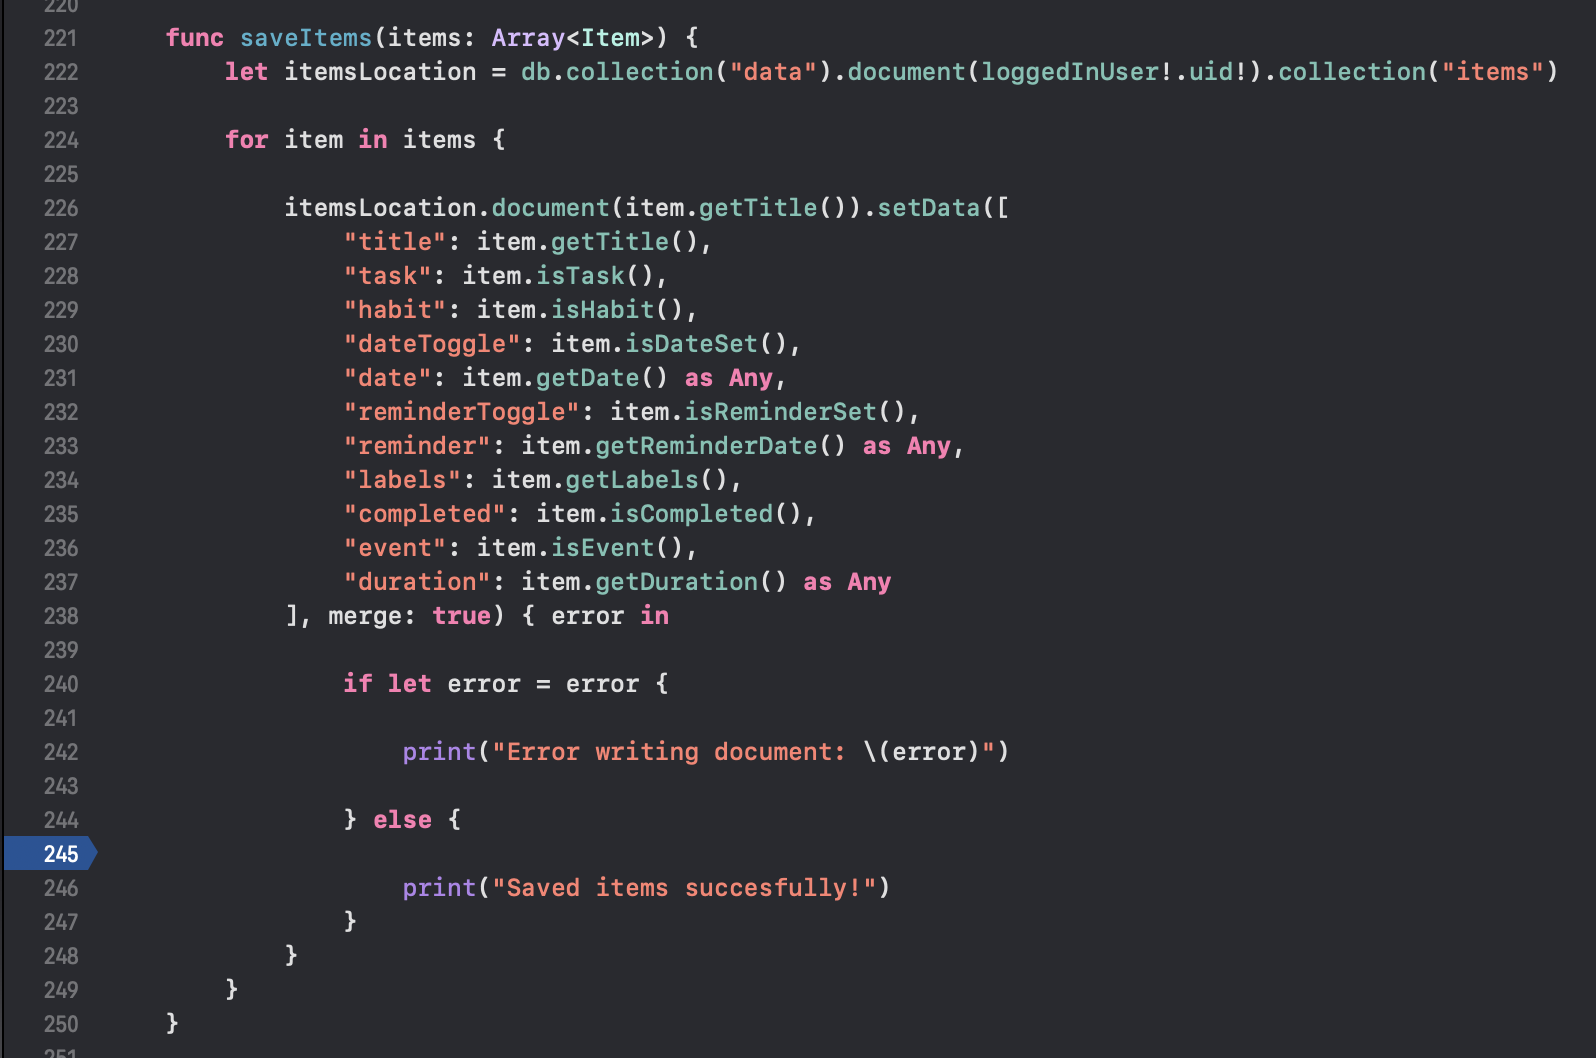
\includegraphics[width=\textwidth]{./graphics/Implementation/Dashboard/firebasesession3.png}
    \caption{saveItems() function defined in FirebaseSession class.}
    \label{fig:firebasesession3_dashboard}
\end{figure}

\begin{figure}[H]
    \centering
    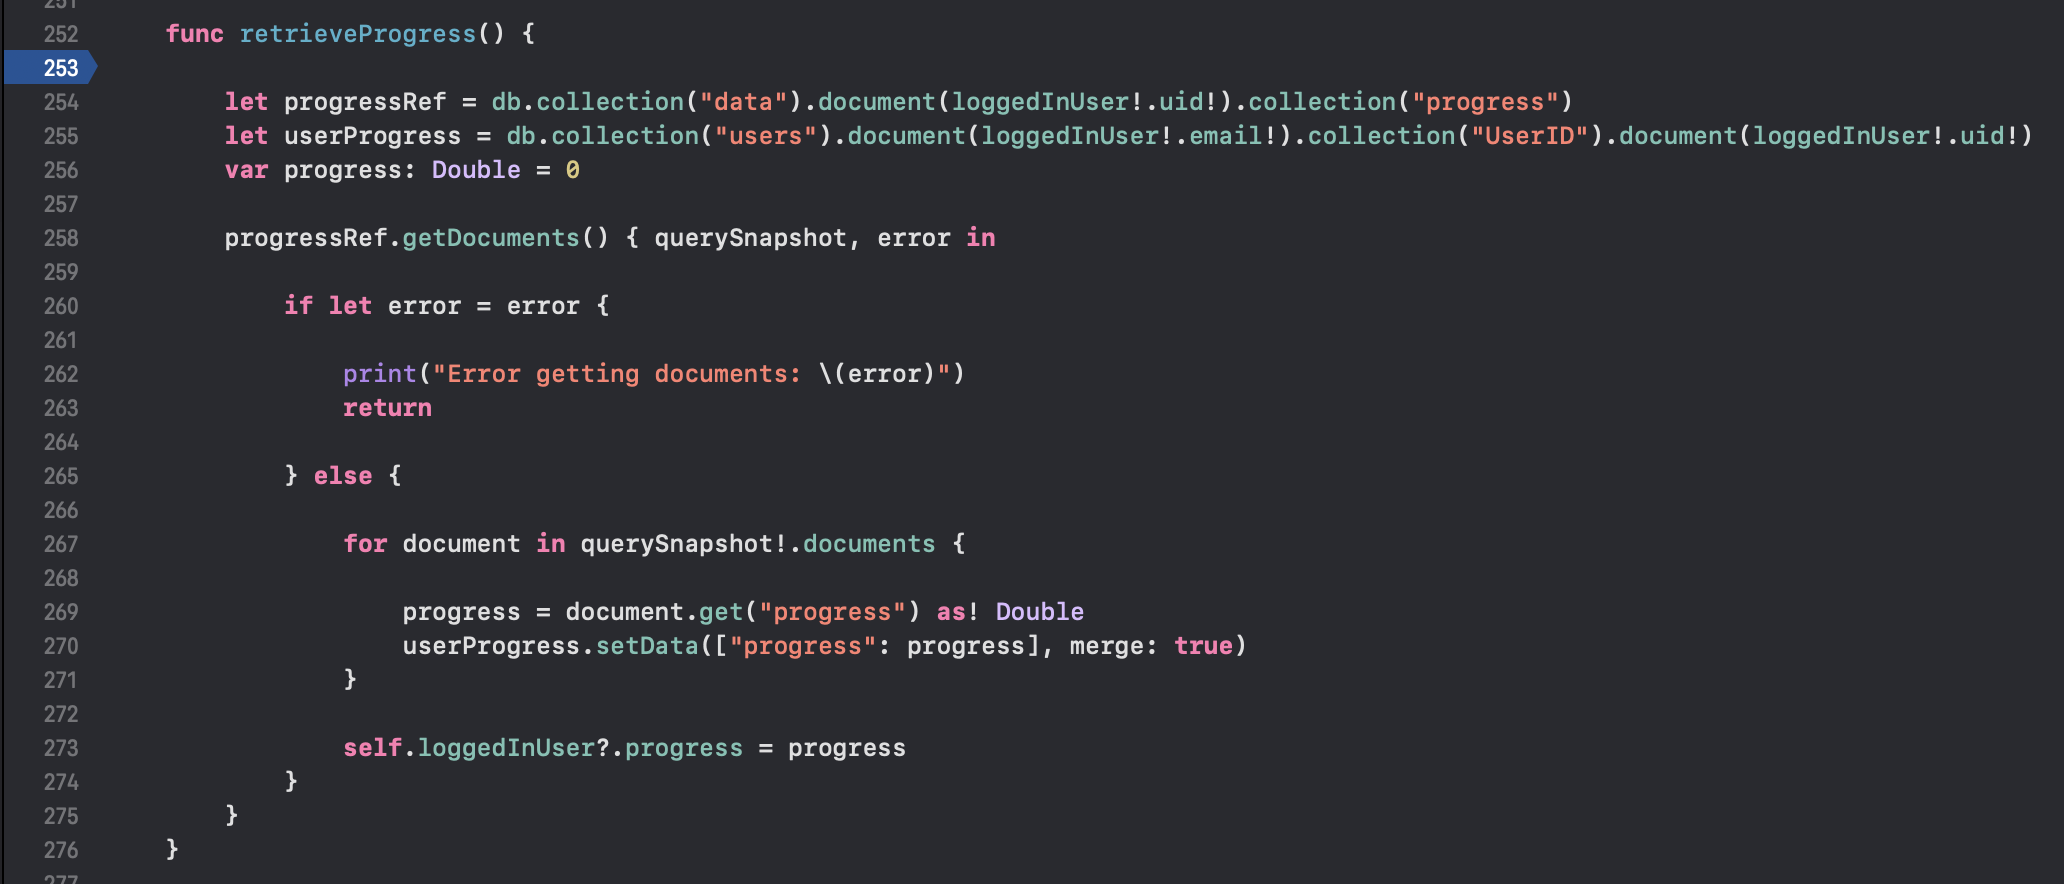
\includegraphics[width=\textwidth]{./graphics/Implementation/Dashboard/firebasesession4.png}
    \caption{retrieveProgress() function defined in FirebaseSession class.}
    \label{fig:firebasesession4_dashboard}
\end{figure}

\begin{figure}[H]
    \centering
    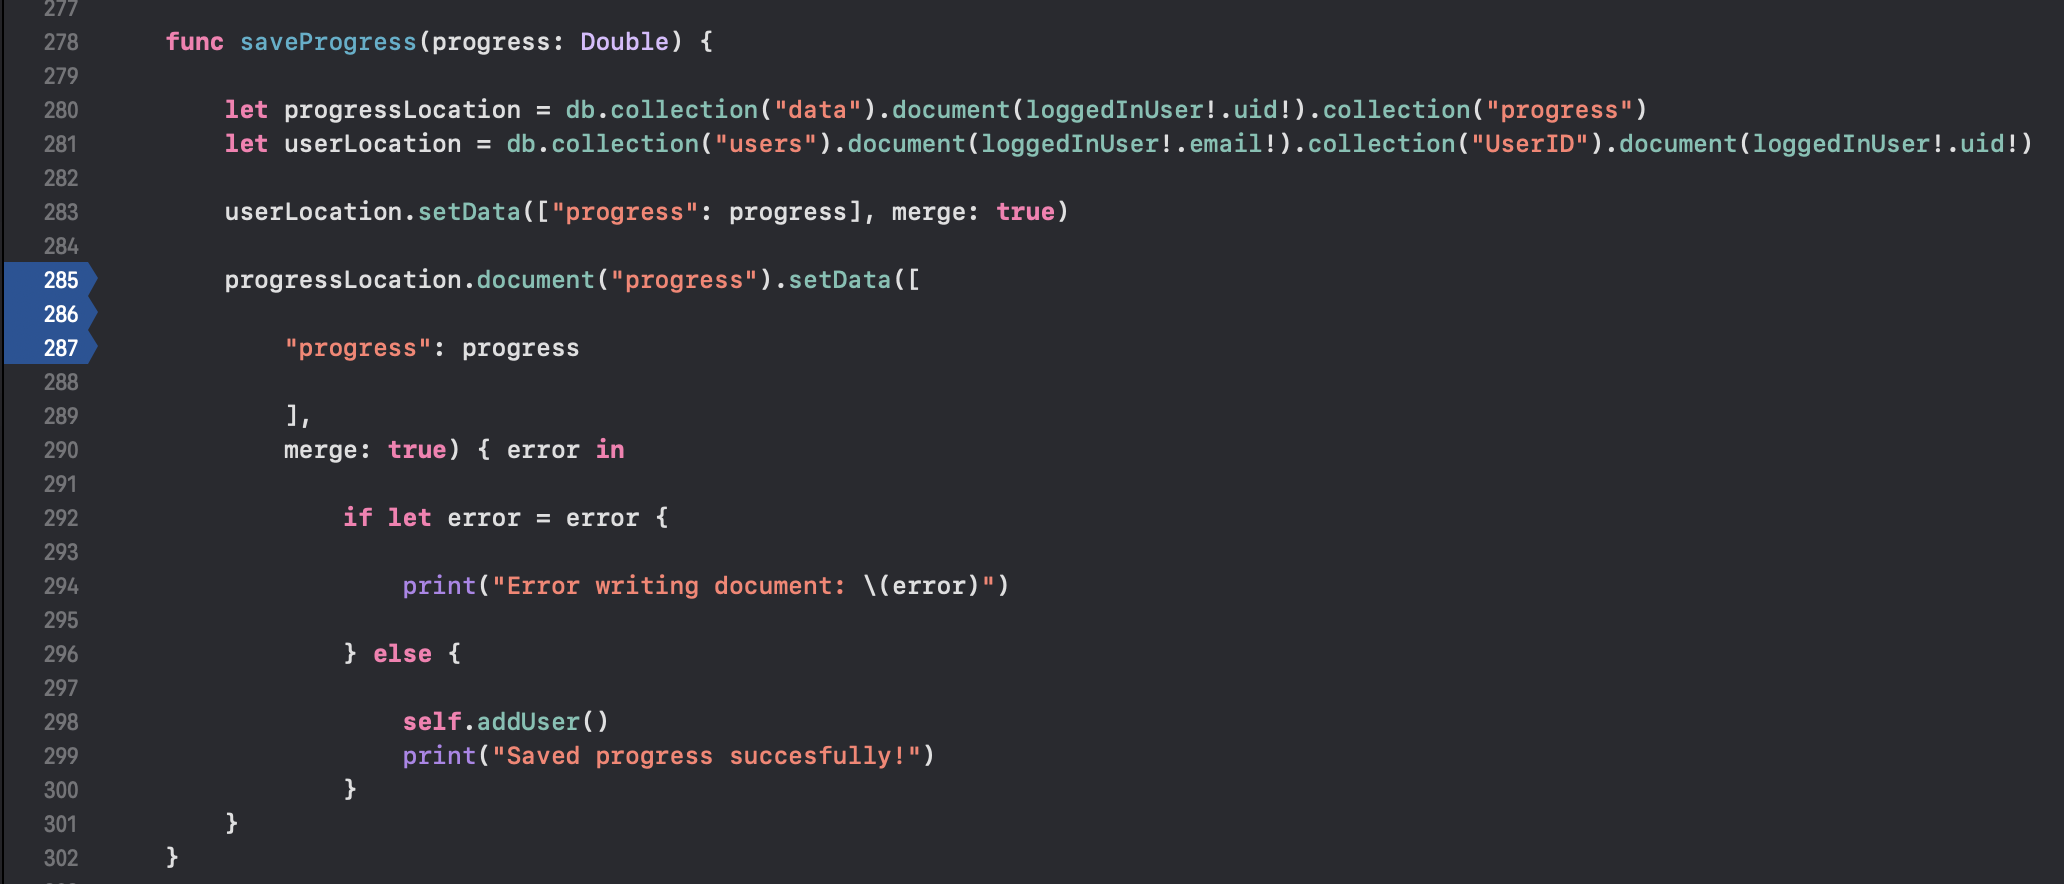
\includegraphics[width=\textwidth]{./graphics/Implementation/Dashboard/firebasesession5.png}
    \caption{saveProgress() function defined in FirebaseSession class.}
    \label{fig:firebasesession5_dashboard}
\end{figure}

\begin{figure}[H]
    \centering
    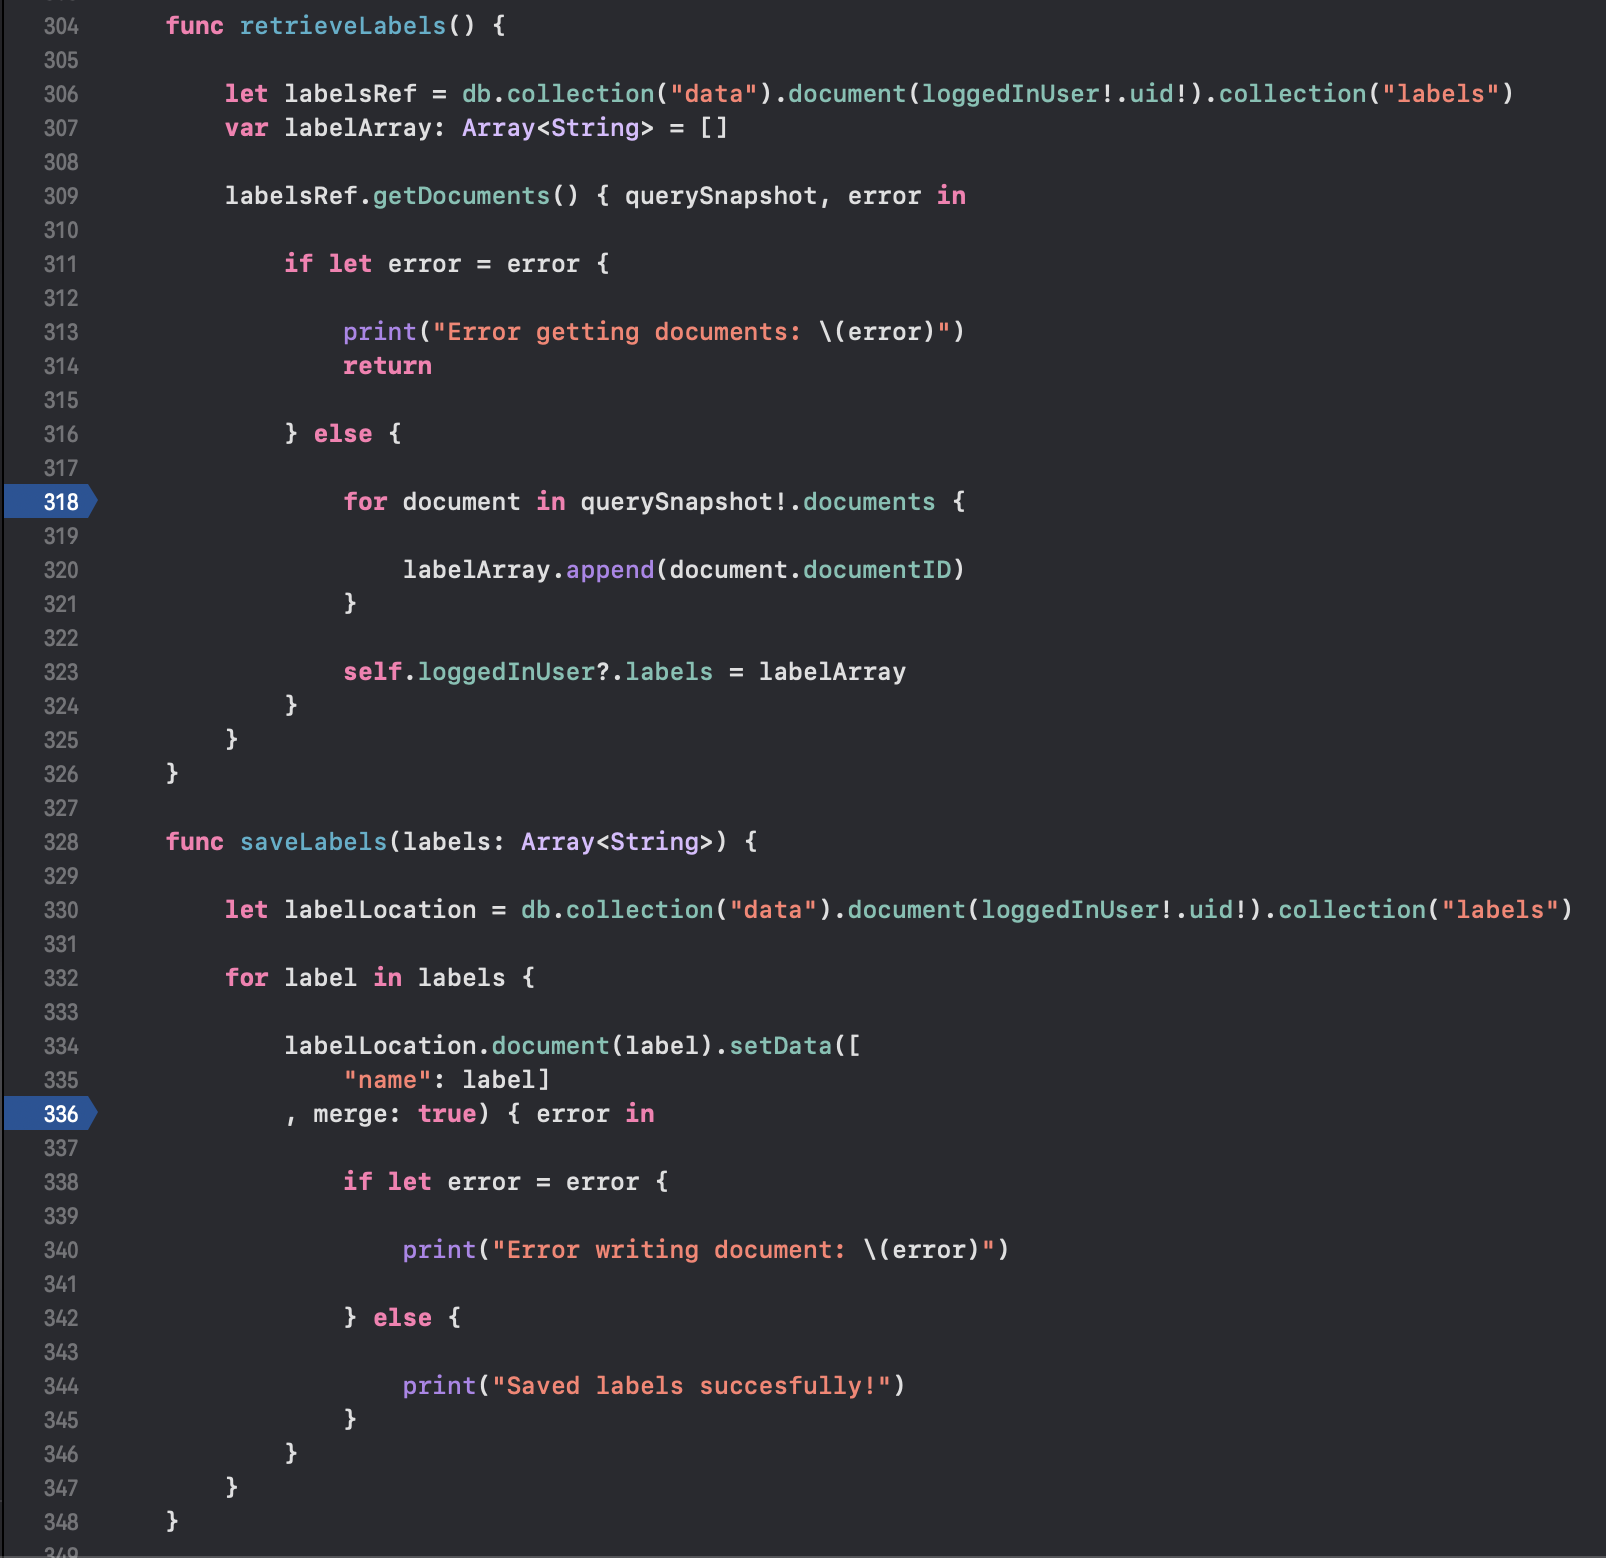
\includegraphics[width=\textwidth]{./graphics/Implementation/Dashboard/firebasesession6.png}
    \caption{retrieveLabels() and saveLabels() functions defined in FirebaseSession class.}
    \label{fig:firebasesession6_dashboard}
\end{figure}

\begin{figure}[H]
    \centering
    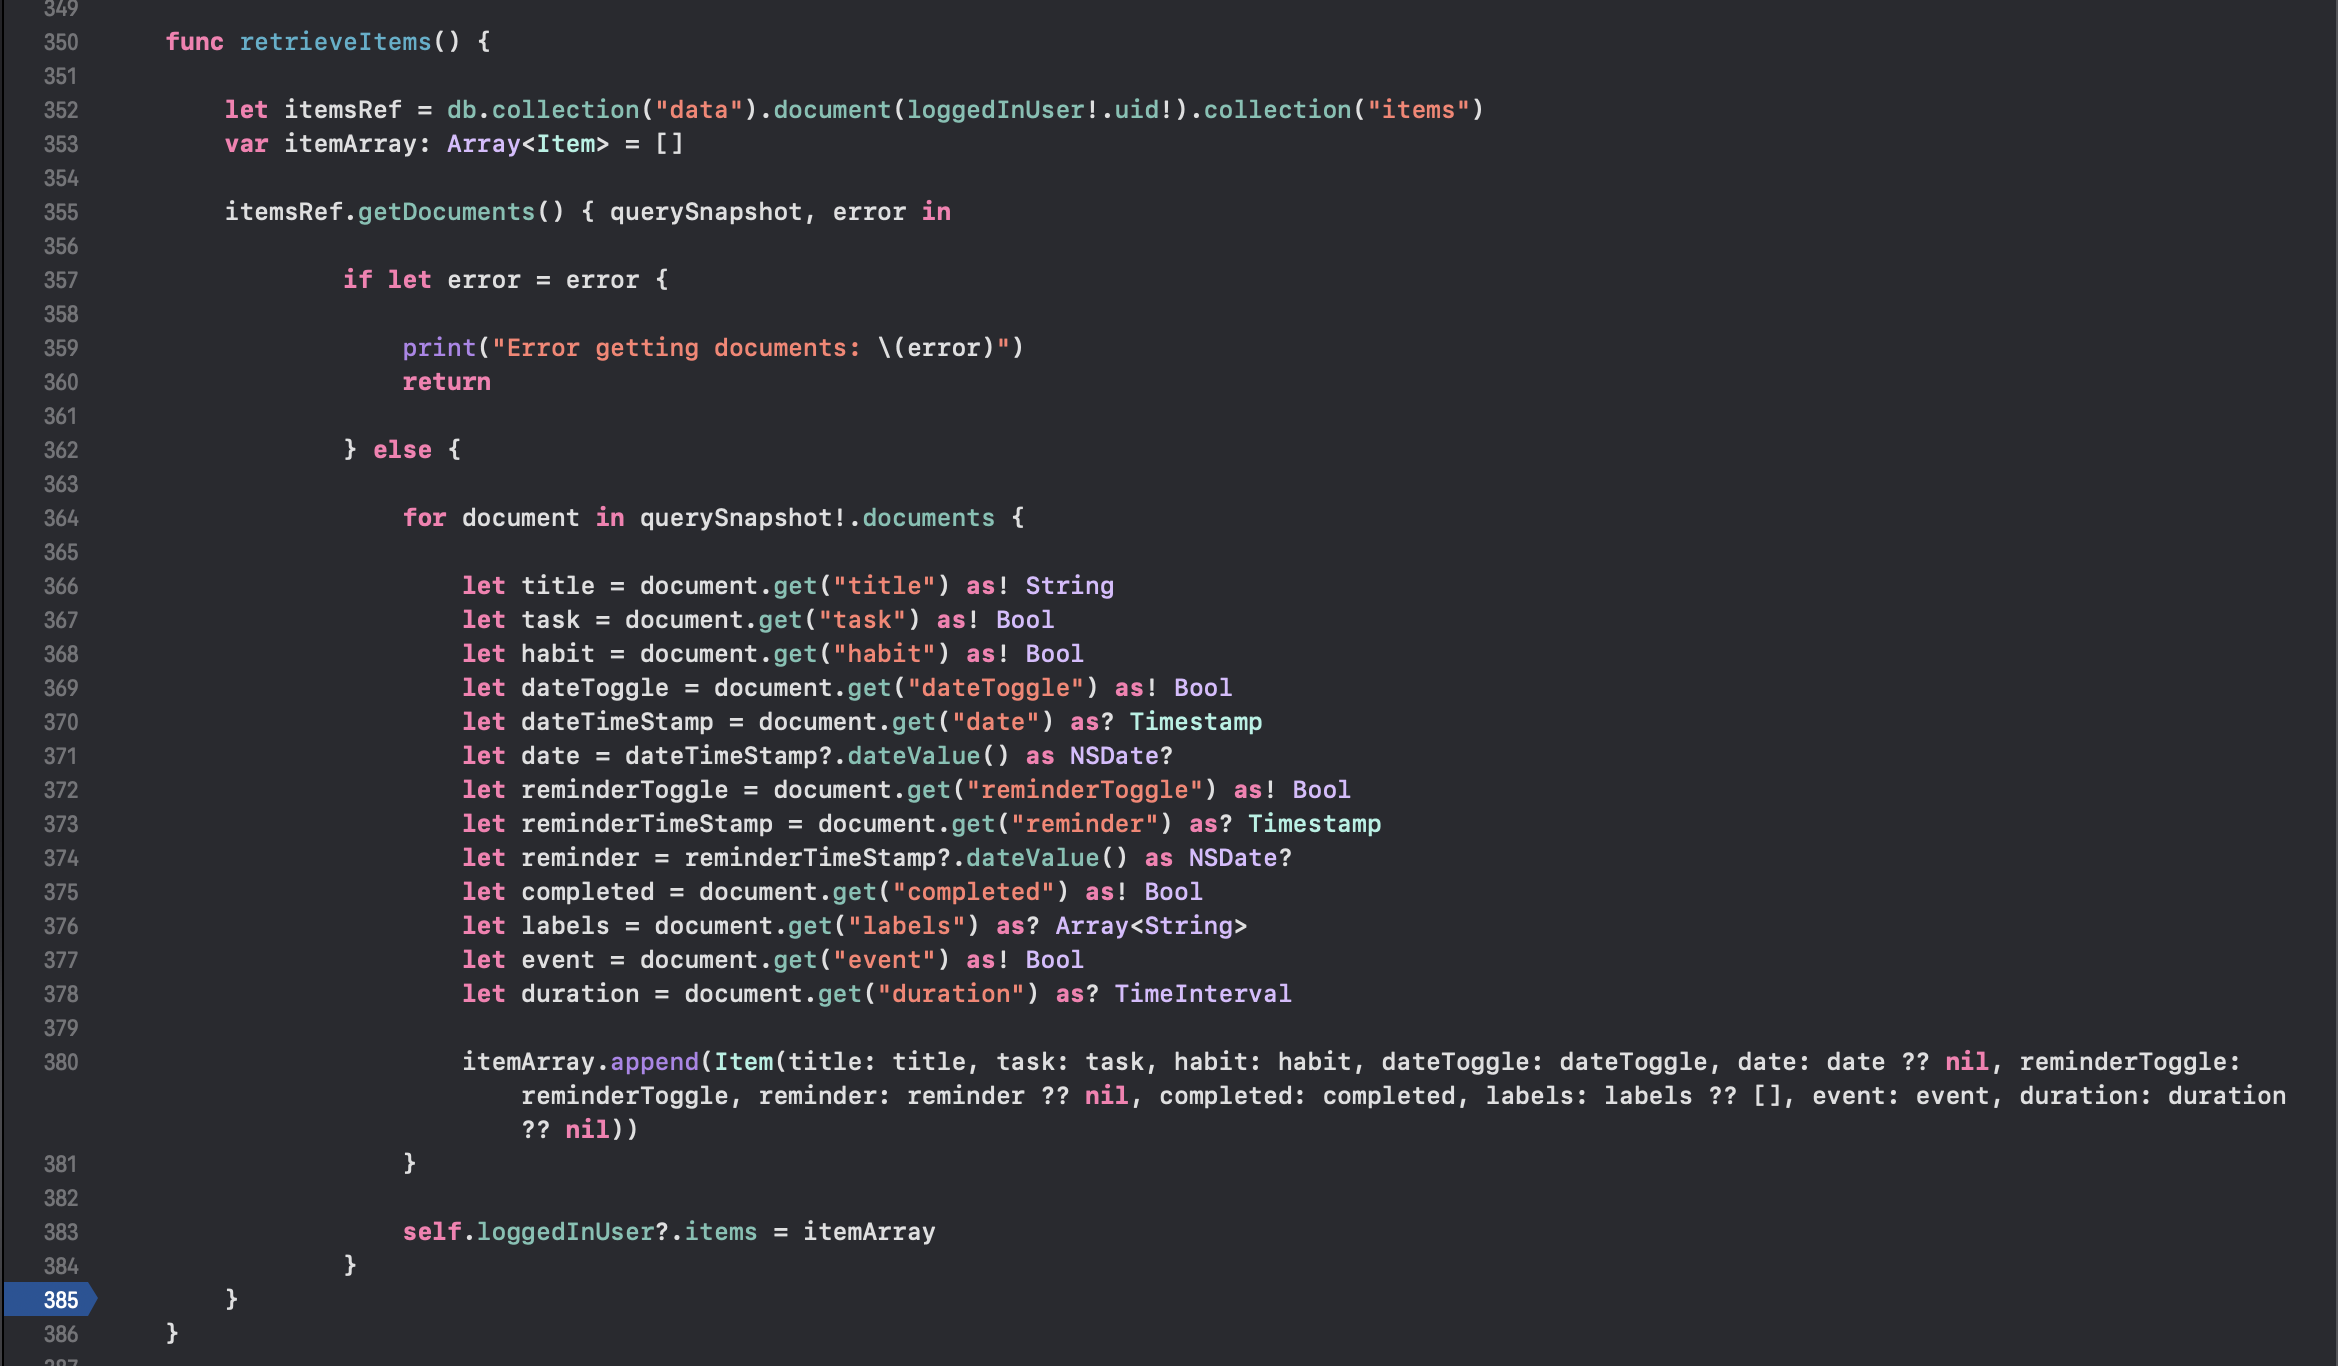
\includegraphics[width=\textwidth]{./graphics/Implementation/Dashboard/firebasesession7.png}
    \caption{retrieveItems() function defined in FirebaseSession class.}
    \label{fig:firebasesession7_dashboard}
\end{figure}

\begin{figure}[H]
    \centering
    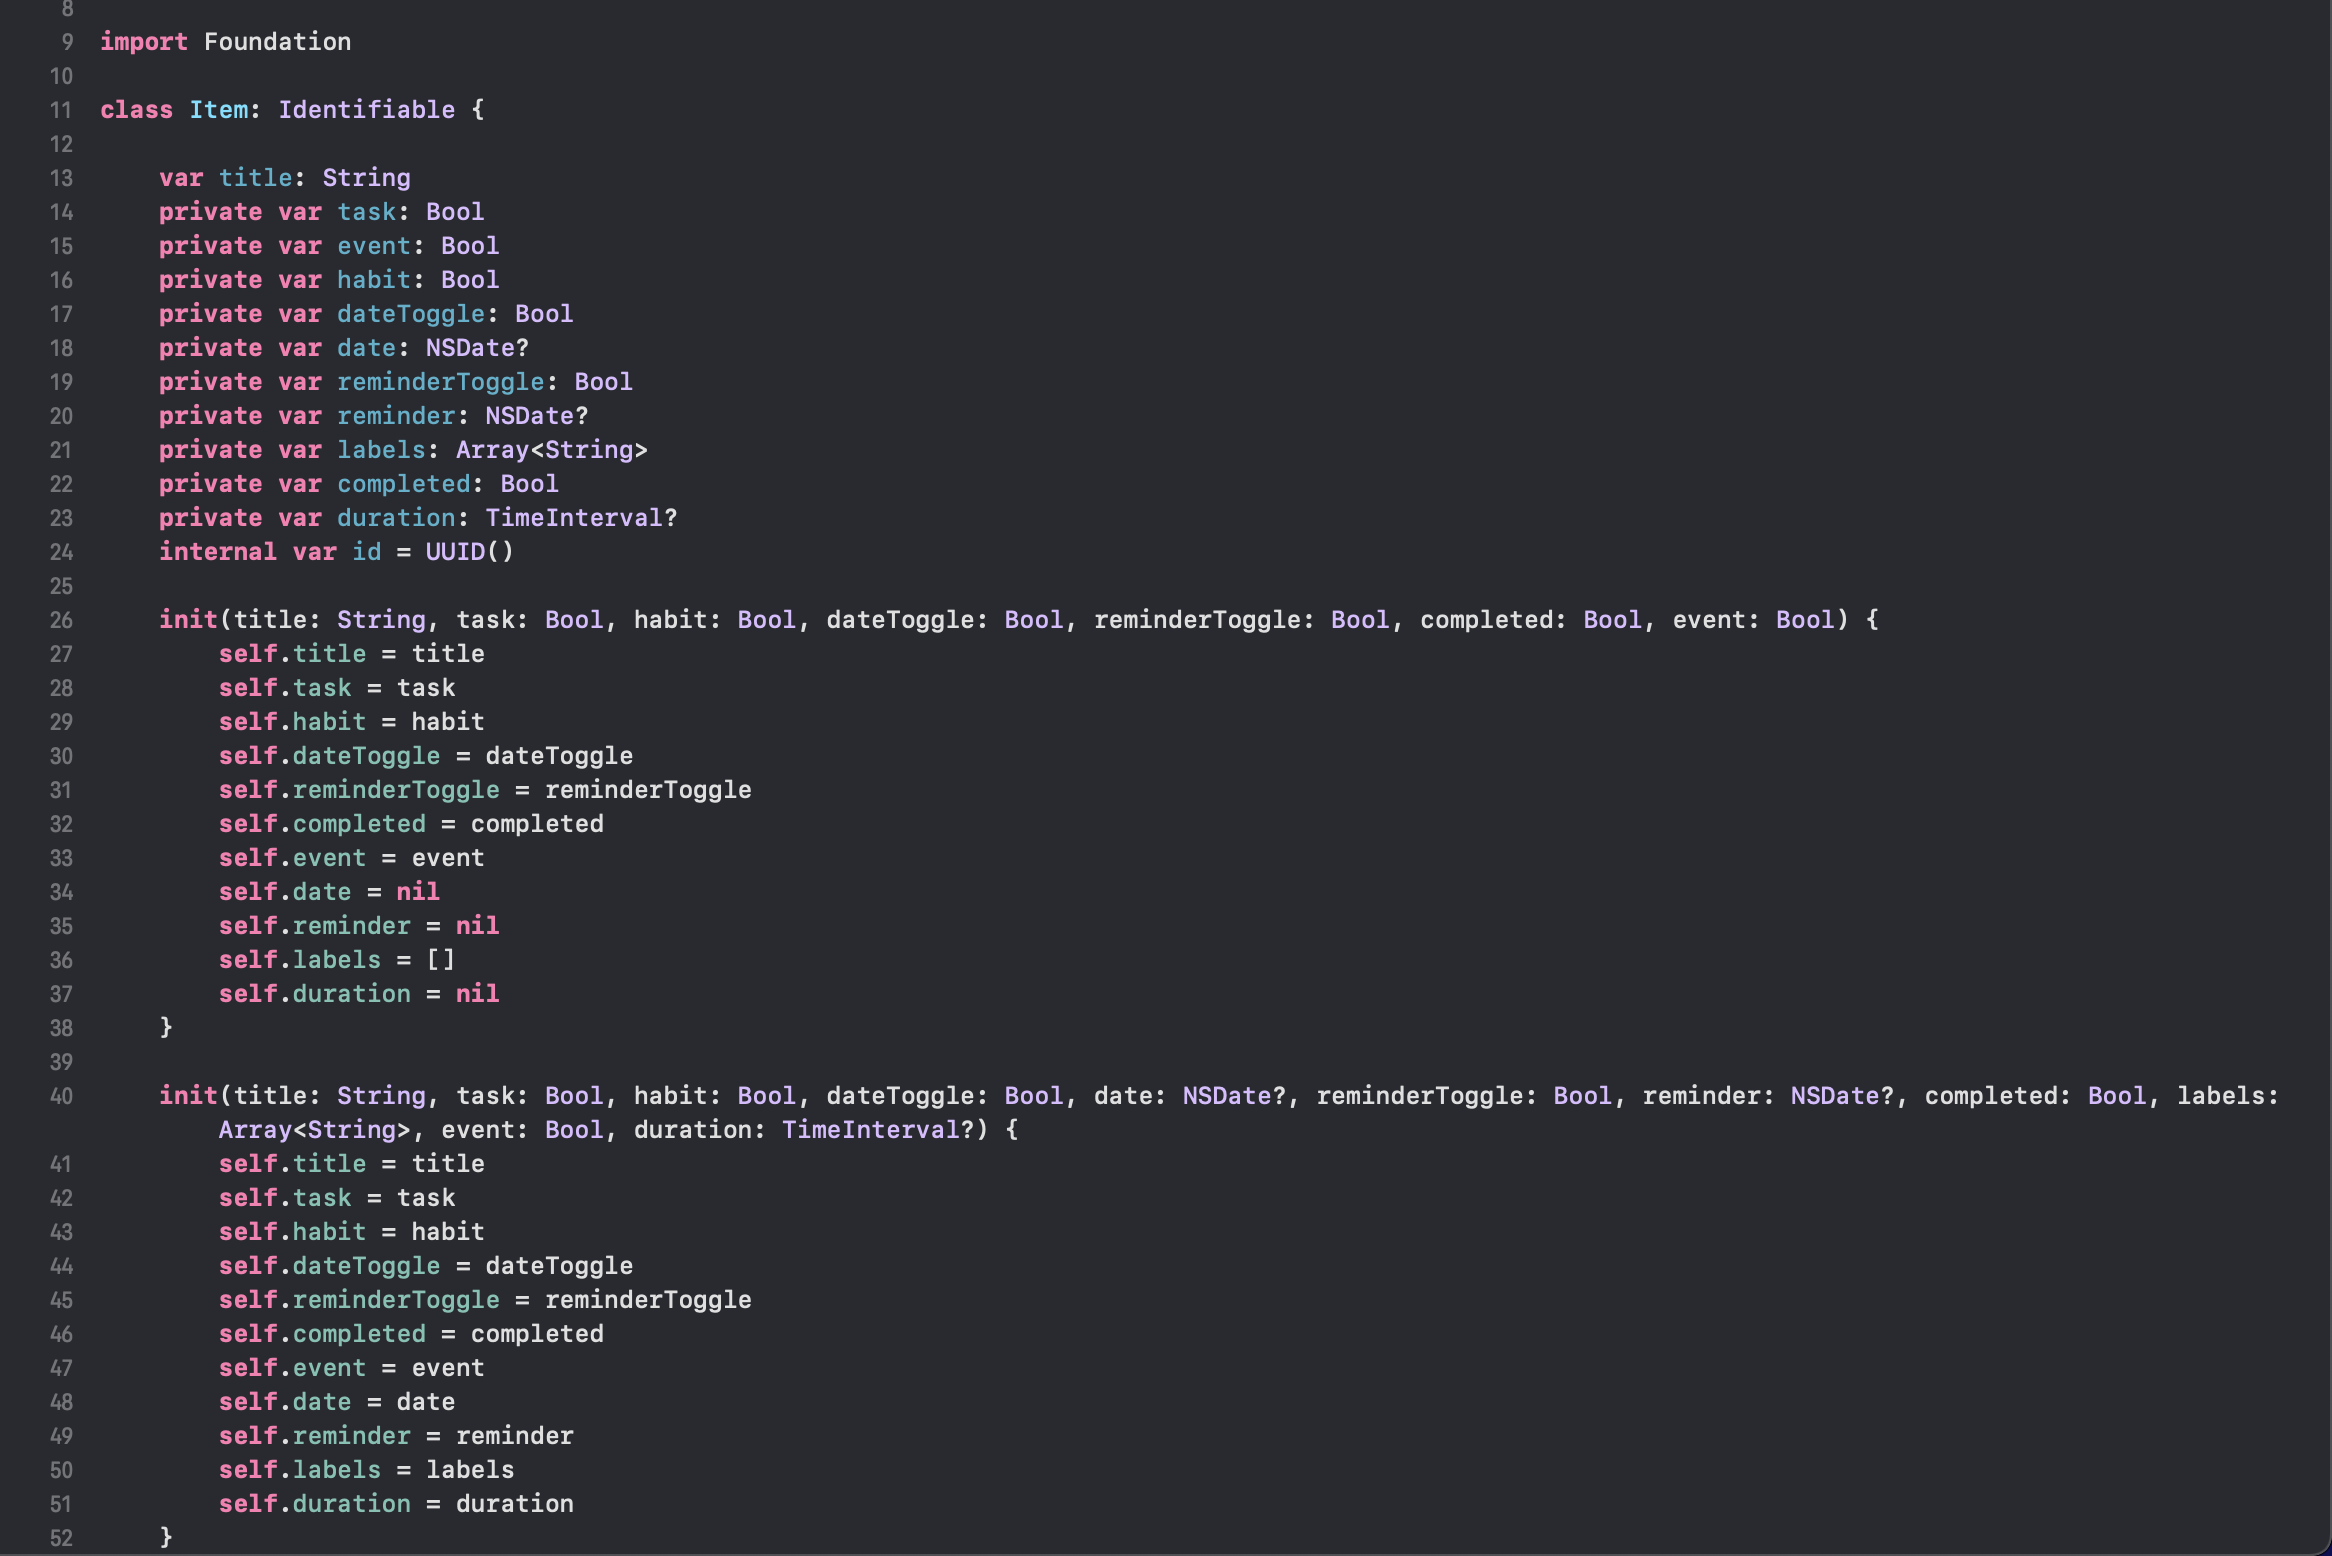
\includegraphics[width=\textwidth]{./graphics/Implementation/Dashboard/item1.png}
    \caption{public variables and constructors defined in Item class.}
    \label{fig:item1}
\end{figure}

\begin{figure}[H]
    \centering
    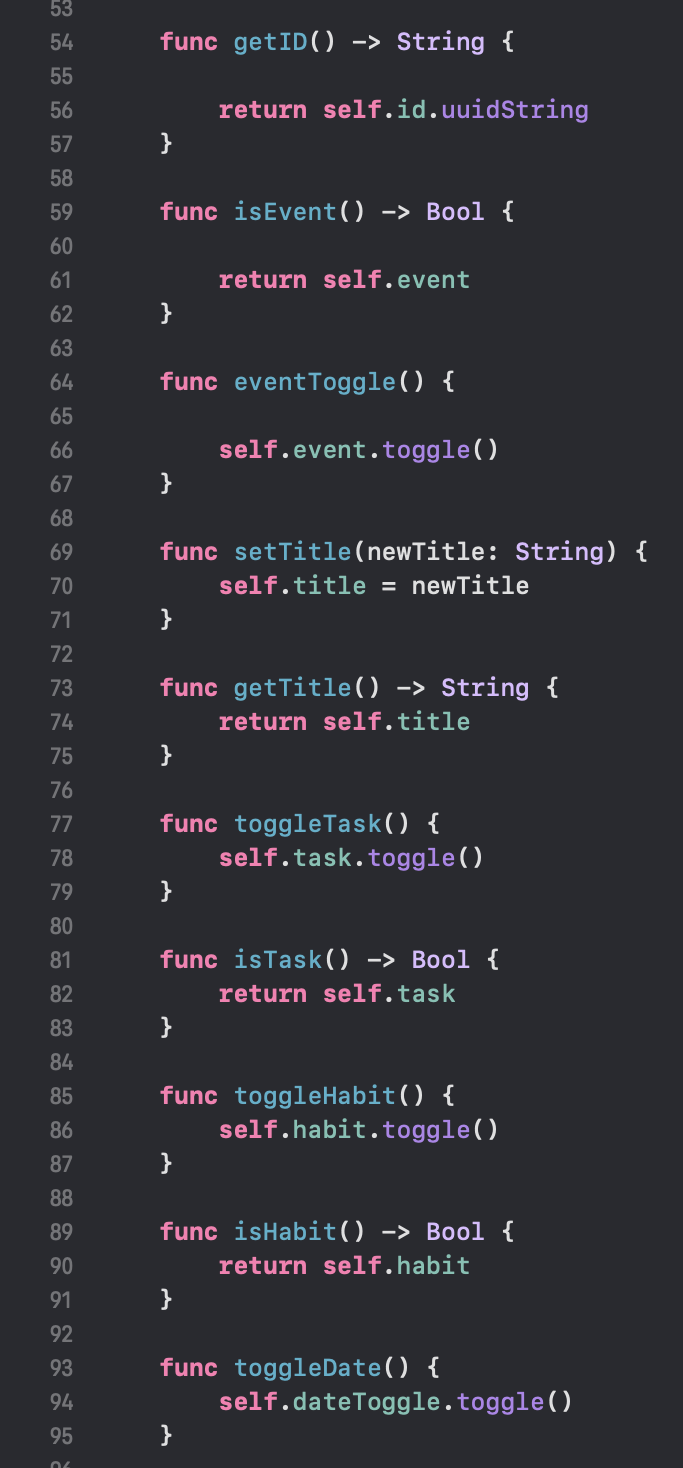
\includegraphics[width=9cm]{./graphics/Implementation/Dashboard/item2.png}
    \caption{Getter and Setter functions defined in Item class.}
    \label{fig:item2}
\end{figure}

\begin{figure}[H]
    \centering
    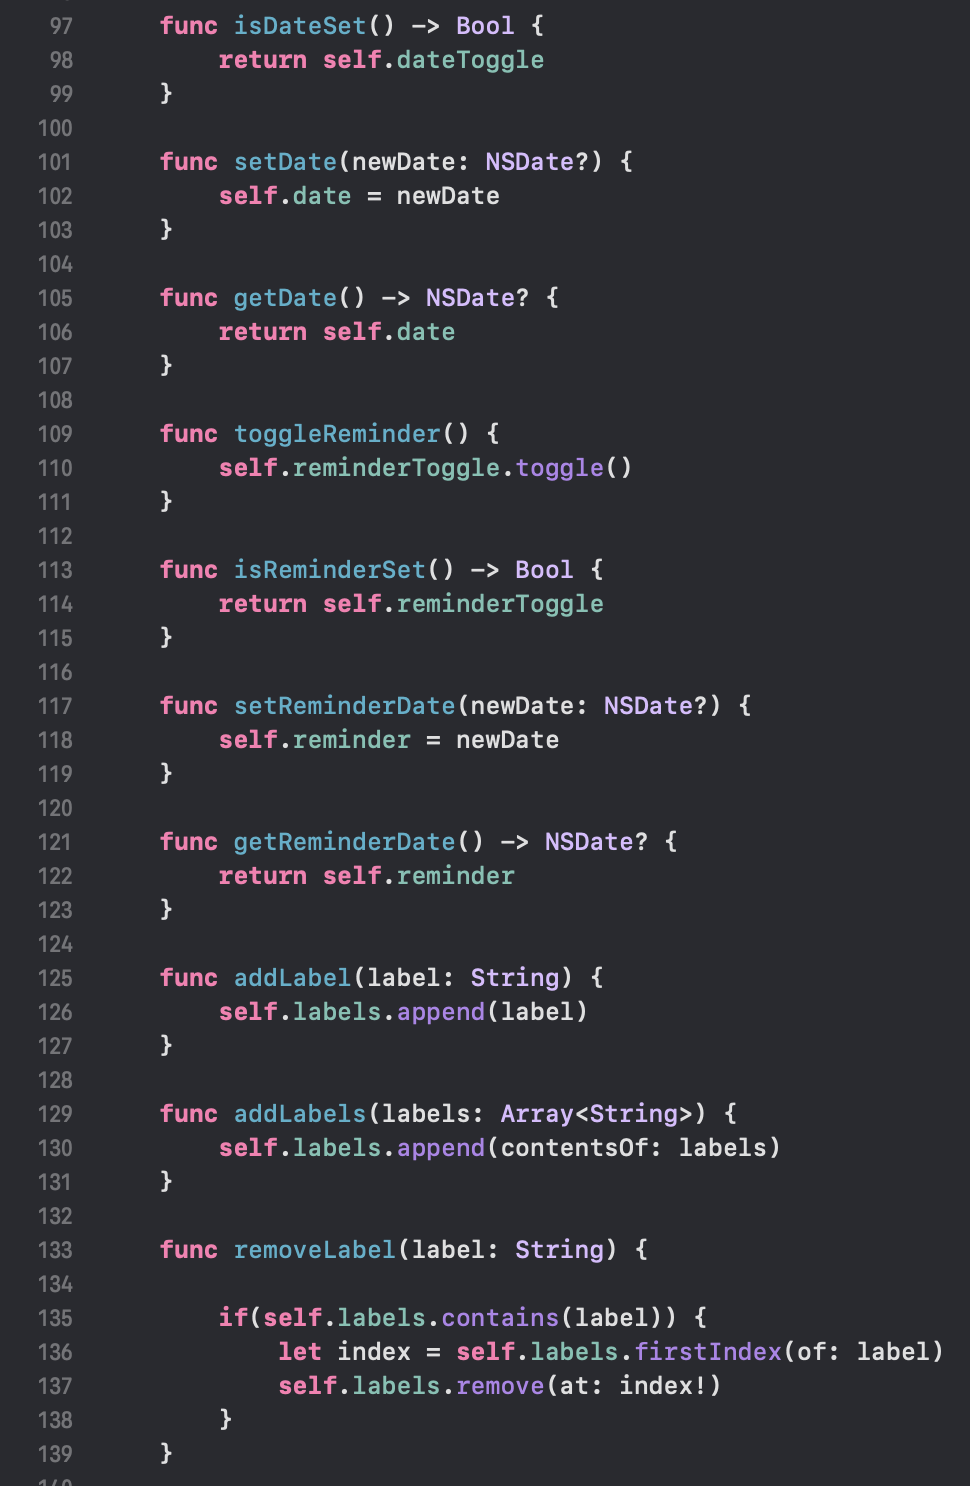
\includegraphics[width=\textwidth]{./graphics/Implementation/Dashboard/item3.png}
    \caption{Getter and Setter functions defined in Item class.}
    \label{fig:item3}
\end{figure}

\begin{figure}[H]
    \centering
    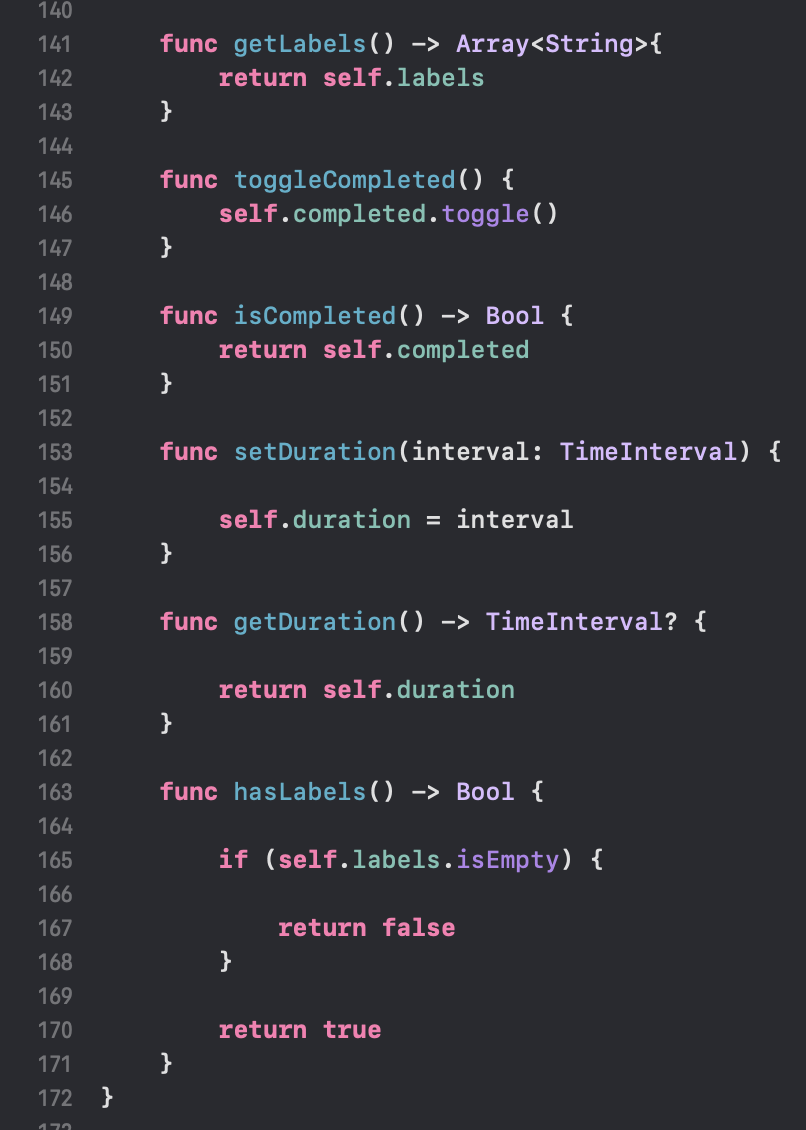
\includegraphics[width=\textwidth]{./graphics/Implementation/Dashboard/item4.png}
    \caption{Getter and Setter functions defined in Item class.}
    \label{fig:item4}
\end{figure}